\section{Parameter Estimation}
\label{sec:estimation}

\subsection{Reference and Metric}
\label{sec:reference}

All constants are fitted to, or inverted from, output measurements of the public Mixbox~2.0 API \texttt{lerpFloat}, using the sRGB display-value float path. The reference is loaded from the official distribution for research comparison only. The metric is CIEDE2000 \cite{sharma2005} with $k_{L}=k_{C}=k_{H}=1$, validated against the 34 reference pairs of Sharma et al.\ (maximum absolute deviation $4.95\times10^{-5}$). Mixing is performed on display values without linearization; $\Delta E_{00}$ is computed after conversion to CIELAB under D65.

\subsection{Inversion Measurements}
\label{sec:inversion}

The design is driven by measurements that invert the reference rather than by assumptions about pigment physics. For each anchored color pair, the per-channel exponent required by a power-law trajectory is read from the reference output at progress $\alpha$:
\begin{equation}
p_{c}(\alpha)=\frac{\ln\bigl((r_{c}-v_{c})/(1-v_{c})\bigr)}{\ln\alpha},
\label{eq:inversion}
\end{equation}
where $v_{c}$ is the pigment channel value and $r_{c}$ the reference output.

Three structural observations follow (\cref{app:inversion} reports the supporting tables). First, the inverted exponent is approximately constant in $\alpha$: it drifts by less than 0.2 over $\alpha\in[0.1,0.9]$ in every family, which supports a single-exponent model; the drift near $\alpha\to1$ is the region addressed by the $\varphi$ map. Second, the exponent decreases with the channel value in a two-step pattern---dark segments hold absorption, bright segments advance quickly---which is the empirical basis of \cref{eq:staircase}. Third, the residual structure is family- and channel-dependent: near-zero channels depend on the channel rather than on the pigment, red-family pigments hold their green absorption when brightened, and complementary mixtures leave a residual of approximate shape $4a(1-a)$ in the middle of the range. These observations motivate the residual, coupling, directional, and harmonic terms of \cref{sec:repair}.

\Cref{fig:staircase} plots the inverted exponents at $\alpha=0.5$ together with the soft-step approximations and the end-to-end inversion of the PBM output.

\begin{figure}[t]
\centering
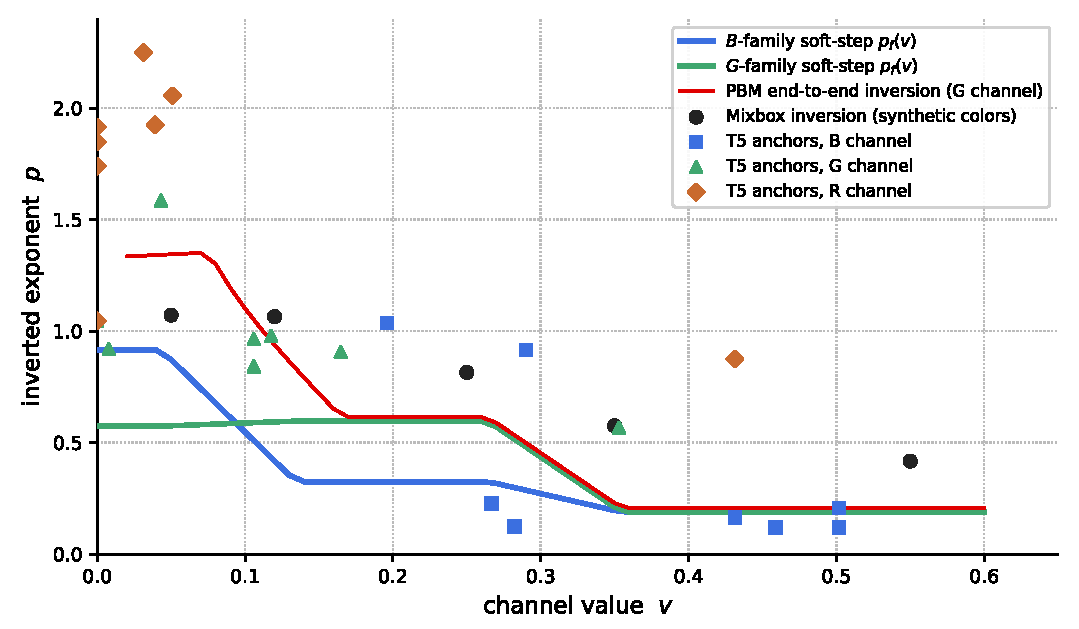
\includegraphics[width=0.78\linewidth]{fig3-staircase.pdf}
\caption{Inverted exponent $p$ at $\alpha=0.5$ as a function of the channel value $v$. Points: Mixbox inversion for synthetic colors and T5 anchors. Lines: the $B$- and $G$-family soft-step approximations and the end-to-end inversion of the PBM output (G channel).}
\label{fig:staircase}
\end{figure}

\subsection{Fitting Procedure}
\label{sec:fitting}

The estimation is two-stage and fully reproducible from the repository tooling.

\paragraph{Corpus.}
The fitting corpus contains the palette suite (T1), the stress-pair suite (T2), the first 800 random pairs of the T3 draw (seed 20260808), the dark-plus-white suite (T5), the two-sided tail suite (T5E), 6000 pseudo-random sRGB pairs (seed 999), and twelve anchored complementary pairs sampled at nineteen ratios; the anchored pairs carry a weight of ten so that the harmonic correction is fitted where it acts.

\paragraph{Harmonic coefficients.}
Because $\hat{\gamma}$ enters \cref{eq:harmonic} linearly, the 51 coefficients are obtained in closed form. For each corpus entry the two role branches contribute
\begin{equation}
\mathbf{y}=
\mathbf{r}-\mathbf{C}-\sum_{b}\lambda_{b}\,g_{b}\,(T_{b}-\mathbf{C}),
\qquad
\mathbf{A}=\sum_{b}\lambda_{b}\,g_{b}\,V_{b},
\label{eq:design}
\end{equation}
where $\mathbf{r}$ is the reference output and the sum runs over the one or two active branches; the coefficients solve the linear least-squares problem $\mathbf{A}\mathbf{w}\approx\mathbf{y}$ per channel, with a ridge of $10^{-6}$. Entries whose total gain $\sum_{b}\lambda_{b}g_{b}$ is below 0.02 are excluded, which leaves 4664 design rows.

\paragraph{Scalars.}
The remaining fourteen scalars---the two staircase positions, the three $B$-family levels and the shared upper level, the coupling amplitude and slope, the gate threshold, slope, and chroma-range threshold, the two envelope constants, the endpoint-compression exponent, and the residual amplitude---are refined by coordinate descent on the in-sample loss
\begin{equation}
L=\overline{\Delta E_{00}}+0.02\,\max\Delta E_{00}+\frac{1}{12}\cdot\overline{\Delta E_{00}}\big|_{\text{anchors}},
\label{eq:loss}
\end{equation}
where the first two terms are evaluated over T1, T2, the 800 fitting pairs of T3, and T5. One alternation is performed: the harmonic coefficients are re-fitted on the updated core, and the change is below 0.014 $\Delta E_{00}$ on every suite, i.e.\ the two stages have reached a fixed point. The fitted constants were then re-evaluated on held-out draws that were not used in fitting (\cref{sec:results}).

\paragraph{Structural simplifications adopted on measured evidence.}
The staircase slope is merged into the shared gate slope; the $G$ and $B$ upper staircase levels share one value; the $\varphi$ width shares $E_{W}=0.08$; the role signal is the maximum channel; and the residual envelope is the $C^{1}$ quadratic of \cref{eq:residual} rather than a piecewise-linear interpolation.

\subsection{Gate Sensitivity}
\label{sec:sensitivity}

To test whether the gate thresholds are tuned to a narrow optimum, each gate threshold and the shared slope $k$ were perturbed by $\pm10\%$ and $\pm20\%$ while all other parameters remained fixed (\cref{tab:sensitivity}). The mean $\Delta E_{00}$ changes by at most 0.11 on T5 and 0.05 on T3. The T5 mean is flat under $w_{0}$ and $\mathrm{maxd}_{0}$ perturbations and moves by at most 0.11 when $k$ is scaled; the T3 maximum grows from 19.4 to 25.2 at $w_{0}\times0.8$, because a small number of complementary pairs are sensitive to the gate boundary. The thresholds therefore sit on a plateau of the loss rather than at a knife edge.

\begin{table}[t]
\centering
\small
\caption{Gate-parameter sensitivity: change in mean $\Delta E_{00}$ ($\Delta$T5 / $\Delta$T3) under $\pm10\%$ and $\pm20\%$ perturbation of each fitted gate parameter, with all other parameters fixed.}
\label{tab:sensitivity}
\begin{tabular}{lcccc}
\toprule
Parameter & $\times0.8$ & $\times0.9$ & $\times1.1$ & $\times1.2$ \\
\midrule
$w_{0}$ (0.37375181) & $+0.000/-0.045$ & $+0.000/-0.023$ & $+0.000/+0.026$ & $+0.000/+0.081$ \\
$\mathrm{maxd}_{0}$ (0.06479933) & $-0.011/-0.003$ & $-0.007/-0.002$ & $+0.010/+0.002$ & $+0.025/+0.005$ \\
shared slope $k$ (11.0163945) & $+0.105/-0.001$ & $+0.029/-0.001$ & $+0.013/+0.002$ & $+0.038/+0.005$ \\
\bottomrule
\end{tabular}
\end{table}
